% Copyright 2026 Sreeram Anil
% SPDX-License-Identifier: CC-BY-4.0
% =============================================================================
%  Super-twisting (second-order sliding-mode) observer
% =============================================================================
\chapter{Super-Twisting Sliding-Mode Observer (SuperTwisting-SMO)}
\label{ch:supertwistingsmo}

\section*{At a glance}
\begin{tabular}{@{}l>{\raggedright\arraybackslash}p{0.76\textwidth}@{}}
Family & Deterministic observers \\
Header & \texttt{include/estkit/observers/super\_twisting.hpp} \\
Registered name & \texttt{SuperTwisting-SMO} \\
State dimension & $n_x + 1 = 5$ (4 model states + 1 injection integrator); $n_y = 1$ \\
Cost per step & $\mathcal{O}(n_x)$, one square root; $\approx 0.14\,\mu$s/step --- cheapest in the study \\
Primary references & \cite{levant1993,davila2005,moreno2008,moreno2012strict,utkin1992} \\
\end{tabular}

\section{Motivation and aerospace/BMS relevance}
The first-order sliding-mode observer of \Cref{ch:smo} pays for its robustness with chattering:
the injection is discontinuous, so either the estimate chatters or a boundary layer is introduced
and exactness is lost.  Levant's super-twisting algorithm \cite{levant1993} resolves the dilemma.
It is a second-order sliding-mode algorithm: the discontinuity is moved into the \emph{derivative}
of the injection, so the injection itself is continuous while the surface $s=0$ and its derivative
$\dot{s}=0$ are both reached in finite time.  Davila, Fridman and Levant \cite{davila2005} turned
it into an observer for mechanical systems; Moreno and Osorio
\cite{moreno2008,moreno2012strict} supplied the strict Lyapunov function that makes the gain
conditions explicit rather than folklore.

For a battery the practical consequences are three.  The injection is continuous, so the SOC
estimate is smooth enough to feed a power-limit calculation without filtering.  The integral part
of the injection provides exactly the same steady-state authority as integral action, so slow
offsets are absorbed.  And the algorithm needs no linear gain and no pole placement at all: it
needs one injection direction and two scalars.  On a flight computer that is about as small as a
model-based SOC estimator gets --- the measured cost here, $0.14\,\mu$s/step, is under a third of
the EKF's.

\section{Problem statement and assumptions}
Plant \eqref{eq:lue-plant-f}--\eqref{eq:lue-plant-h}, $n_y=1$, sliding variable $s = r$ as in
\eqref{eq:smo-s}.
\begin{assumption}[Lipschitz-in-time perturbation]\label{as:sto-pert}
The lumped perturbation $\varrho$ acting on the sliding variable satisfies the growth bound
\begin{equation}
|\varrho(t)| \le \delta\,|s|^{1/2} ,
\label{eq:sto-growth}
\end{equation}
for a known $\delta>0$.  This is weaker than requiring $\varrho$ bounded near $s=0$ and is the
condition under which the super-twisting algorithm is exactly convergent
\cite{moreno2008}.
\end{assumption}

\section{Derivation}

\subsection{The algorithm}
In continuous time the super-twisting pair is
\begin{align}
\dot{s} &= -k_{1c}|s|^{1/2}\sgn(s) + \zeta + \varrho(t) , \label{eq:sto-c1}\\
\dot{\zeta} &= -k_{2c}\sgn(s) . \label{eq:sto-c2}
\end{align}
Both right-hand sides are discontinuous only in $\dot\zeta$; the injection
$\nu = k_{1c}|s|^{1/2}\sgn(s) + \zeta$ that enters the plant is continuous.  Discretising with
the sample time $\dt$ and writing $k_1 = k_{1c}\dt$, $k_2 = k_{2c}\dt^2$ gives the implemented
observer
\begin{align}
\xminus_k &= f(\xplus_{k-1},\vu_{k-1}) , \label{eq:sto-pred}\\
r_k &= y_k - h(\xminus_k,\vu_k) , \label{eq:sto-res}\\
\nu_k &= k_1|r_k|^{1/2}\sgn(r_k) + w_k , \label{eq:sto-nu}\\
\xplus_k &= \xminus_k + \bm{\Lambda}\,\nu_k , \label{eq:sto-upd}\\
w_{k+1} &= \operatorname{sat}\!\big(w_k + k_2\,\sat(r_k/\phi);\ w_{\max}\big) . \label{eq:sto-w}
\end{align}
$\bm{\Lambda}\in\real^{n_x}$ is the injection direction and $w$ the integral part.

\subsection{Gain conditions (Moreno--Osorio)}
Moreno and Osorio \cite{moreno2008,moreno2012strict} construct the strict Lyapunov function
\begin{equation}
V(s,\zeta) = 2k_{2c}|s| + \tfrac12\zeta^2 + \tfrac12\big(k_{1c}|s|^{1/2}\sgn(s) - \zeta\big)^2 ,
\label{eq:sto-lyap}
\end{equation}
which is continuous, positive definite and differentiable everywhere except on $s=0$, and show
that along the trajectories of \eqref{eq:sto-c1}--\eqref{eq:sto-c2} with the perturbation bound
\eqref{eq:sto-growth},
\begin{equation}
\dot{V} \le -\frac{\varsigma}{|s|^{1/2}}\,V
\end{equation}
for some $\varsigma>0$, and hence finite-time convergence to the origin, provided
\begin{equation}
\boxed{\ k_{1c} > 2\delta , \qquad
k_{2c} > k_{1c}\,\frac{5\delta k_{1c} + 4\delta^2}{2\,(k_{1c}-2\delta)}\ }
\label{eq:sto-cond}
\end{equation}
Since $V$ is a quadratic form in $\bm{\varsigma}=[|s|^{1/2}\sgn(s),\ \zeta]^\T$, the settling
time is bounded by $2V(s_0,\zeta_0)^{1/2}/\varsigma$, which is finite and independent of the
size of $\varrho$ within \eqref{eq:sto-growth}.

A convenient sufficient choice, and the one usually quoted from Levant \cite{levant1993}, is
\begin{equation}
k_{1c} = 1.5\sqrt{\delta} , \qquad k_{2c} = 1.1\,\delta .
\label{eq:sto-levant}
\end{equation}
The per-step gains follow from $k_1 = k_{1c}\dt$ and $k_2 = k_{2c}\dt^2$, which is the mapping
\texttt{Options::k1} and \texttt{Options::k2} document.

\subsection{Injection direction}
\label{sec:sto-lambda}
The algorithm acts on a scalar; $\bm{\Lambda}$ says how that scalar reaches the state.  The
implementation normalises so that $\mC\bm{\Lambda} = 1$, which makes the output-error dynamics
exactly \eqref{eq:sto-c1} to first order, and puts the whole injection on the state with the
largest DC disturbance gain:
\begin{equation}
\bm{\Lambda} = \frac{1}{C_{j^\star}}\,\bm{e}_{j^\star} ,
\qquad j^\star = \arg\max_j\norm{(\mI-\mA+\mu\mI)\inv\bm{e}_j}_1 ,
\label{eq:sto-lambda}
\end{equation}
with a floor on $|C_{j^\star}|$ to guard the division.  For the cell this is
$\bm{\Lambda} = (\partial\ocv/\partial\soc)\inv\bm{e}_{\soc}$: all of the injection goes into SOC
and the RC branches are propagated open-loop from the measured current.  That is deliberate and
is the standard structure for SOC sliding-mode observers \cite{kim2006smo}: the RC voltages are
well determined by the known input and a stable, fast dynamics, whereas SOC is the integrator
that needs the measurement.  Because $\mC\bm{\Lambda}=1$ by construction, the scalar analysis of
\eqref{eq:sto-cond} applies directly to the output error, with no cross-coupling factor to
estimate.

\subsection{Boundary layer inside the integrator}
A pure $\sgn(r_k)$ in \eqref{eq:sto-w} makes $w$ a random walk driven by the measurement noise:
over $N$ samples its standard deviation is $k_2\sqrt{N}$, which for $k_2 = 2\times10^{-8}$ and
$N=20\,010$ is $2.8\times10^{-6}$ --- small, but not zero, and it grows as $\sqrt{N}$ forever.
Replacing $\sgn$ by $\sat(r/\phi)$ with $\phi=\sigma_v$ makes the drive proportional to the
\emph{mean} residual inside the layer, so zero-mean noise averages out and only a systematic
residual moves $w$.  This is the same regularisation as in \Cref{ch:smo}, applied only to the
discontinuous part; the injection $\nu$ remains continuous either way.  $w$ is additionally
clamped at $w_{\max}$ (anti-windup).

\section{Algorithm}
\begin{algorithm}[H]
\caption{SuperTwisting-SMO --- one sampling period}
\begin{algorithmic}[1]
\Require $\xplus_{k-1}$, $\vu_{k-1}$, $y_k$, $\vu_k$, integral injection $w$, gains $k_1,k_2$, layer $\phi$
\State \textbf{Time update:} $\xminus_k \gets f(\xplus_{k-1},\vu_{k-1})$; \quad $\hat{y}_k \gets h(\xminus_k,\vu_k)$
\State $\mC \gets \texttt{jac\_H}(\xminus_k,\vu_k)$; \quad $\bm{\Lambda}\gets \bm{e}_{j^\star}/C_{j^\star}$ \eqref{eq:sto-lambda}
\State $r_k \gets y_k - \hat{y}_k$
\State $\nu_k \gets k_1\sqrt{|r_k|}\,\sgn(r_k) + w$ \Comment{continuous injection}
\State $\xplus_k \gets \xminus_k + \bm{\Lambda}\nu_k$
\State $w \gets \operatorname{clamp}\big(w + k_2\sat(r_k/\phi),\ \pm w_{\max}\big)$ \Comment{discontinuity lives here}
\State $\xplus_k \gets \operatorname{constrain}(\xplus_k)$
\Ensure $\xplus_k$, $w$
\end{algorithmic}
\end{algorithm}

\section{Application to the battery model}
With $\bm{\Lambda}$ from \eqref{eq:sto-lambda} the SOC update per sample is
$\Delta\soc = \nu/(\partial\ocv/\partial\soc)$.  Benchmark options: $k_1 = 6\times10^{-4}$,
$k_2 = 2\times10^{-8}$, $\phi = \sigma_v = 2$\,mV, $w_{\max}=2\times10^{-3}$.  Two sanity checks
on those numbers:
\begin{itemize}[nosep]
\item At the noise floor, $|r| \approx 2$\,mV, the continuous term gives
$\Delta\soc \approx 6\times10^{-4}\times0.045/0.8 = 3.4\times10^{-5}$ per sample --- comparable to
the linear observers' $L_{\soc}r \approx 1.3\times10^{-3}\times0.002 = 2.6\times10^{-6}$ times
the square-root amplification, i.e. the square root makes the observer relatively \emph{more}
aggressive at small residuals, which is the characteristic super-twisting signature.
\item At a $0.3$\,V residual (the initial-error transient) the term gives
$\Delta\soc \approx 6\times10^{-4}\times0.548/0.8 = 4.1\times10^{-4}$ per sample, i.e.
$4.1\times10^{-3}$ SOC per second; a $0.35$ SOC error is therefore walked out in of order
$100$\,s, which matches the measured $125$\,s.
\end{itemize}
Translating to \eqref{eq:sto-levant}: $k_{1c} = k_1/\dt = 6\times10^{-3}$ and
$k_{2c} = k_2/\dt^2 = 2\times10^{-6}$, which corresponds to
$\delta \approx (k_{1c}/1.5)^2 = 1.6\times10^{-5}$ --- the perturbation growth coefficient the
design is guaranteed against.  Interpreting \eqref{eq:sto-growth} at the observed residual scale
$|s|\approx 5$\,mV gives $|\varrho|\le \delta|s|^{1/2}\approx 1.1\times10^{-6}$\,V per step, i.e.
$11\,\mu$V/s of admissible drift in the lumped model error; the cell's real drift in the nominal
scenario is well inside that, in \texttt{param\_mismatch} it is not, and the benchmark numbers
reflect exactly that ordering.

\section{Implementation notes}
$4280$ bytes and $0.14\,\mu$s/step, the smallest and fastest estimator in the whole study: there is
no gain design, no Riccati equation, no matrix inverse and no $\mathcal{O}(n_x^3)$ path at all.
The only transcendental is one \texttt{sqrt} per step.  The state added over a pure model
propagation is a single scalar $w$.

The two numerical guards are the clamp on $w$ and the boundary layer inside the $\sgn$.  Note
that $|r|^{1/2}$ has unbounded derivative at $r=0$, which is the source of the algorithm's
strength and, in a fixed-step implementation, of a small limit cycle of amplitude
$\mathcal{O}(k_1^2)$; with $k_1 = 6\times10^{-4}$ that is $\mathcal{O}(10^{-7})$ SOC and
invisible.  The float build reproduces the double build exactly to the printed precision.

Because $\bm{\Lambda}$ is supported on one state, the observer places no correction on the RC and
hysteresis channels; those are driven open-loop by the measured current.  This is a feature when
the current sensor is good (fewer degrees of freedom to corrupt) and a limitation when it is not.

\section{Benchmark results}
% Copyright 2026 Sreeram Anil
% SPDX-License-Identifier: CC-BY-4.0
\begin{table}[H]\centering\footnotesize\setlength{\tabcolsep}{4pt}
\caption{SuperTwisting-SMO: cell-level benchmark on the eVTOL mission (mean over seeds; RMSE and max error in \% SOC; $t_\mathrm{conv}$: first time the error stays below 2\,\% for 60\,s, -- = never; EKF reference: steady-state RMSE of the plain EKF on the same data).}\label{tab:cell_SuperTwistingSMO}
\begin{tabular}{llrrrrrcrr}\toprule
plant & scenario & RMSE & RMSE$_\mathrm{ss}$ & max & $t_\mathrm{conv}$ [s] & RMSE$_v$ [mV] & div. & EKF ref. & ns/step \\ \midrule
ECM & nominal & 0.27 & 0.09 & 1.37 & 0 & 0.79 & no & 0.05 & 142 \\
ECM & init\_error & 5.17 & 0.09 & 34.96 & 125 & 36.49 & no & 0.05 & 142 \\
ECM & current\_bias & 1.26 & 0.99 & 5.37 & 0 & 1.39 & no & 0.61 & 142 \\
ECM & noise\_step & 0.29 & 0.16 & 1.37 & 0 & 1.10 & no & 0.12 & 138 \\
ECM & outliers & 0.27 & 0.09 & 1.37 & 0 & 0.82 & no & 0.21 & 143 \\
ECM & cold & 0.56 & 0.37 & 2.90 & 0 & 1.96 & no & 0.16 & 143 \\
ECM & hot & 0.20 & 0.04 & 0.88 & 0 & 0.54 & no & 0.03 & 141 \\
ECM & aged\_cell & 3.24 & 2.49 & 10.74 & 0 & 13.67 & no & 1.52 & 134 \\
ECM & param\_mismatch & 2.19 & 1.73 & 8.49 & 0 & 6.73 & no & 1.36 & 137 \\
ECM & sensor\_dropout & 0.37 & 0.09 & 3.31 & 0 & 0.91 & no & 0.46 & 142 \\
ECM & preisach & 1.16 & 1.10 & 3.26 & 227 & 1.14 & no & 0.20 & 142 \\
ECM & combined & 4.37 & 2.46 & 24.97 & 91 & 29.51 & no & 12.44 & 133 \\
\midrule
SPM & nominal & 1.03 & 0.96 & 4.21 & 0 & 2.80 & no & 3.73 & 133 \\
SPM & init\_error & 5.32 & 0.96 & 34.96 & 201 & 35.53 & no & 3.81 & 132 \\
SPM & current\_bias & 1.27 & 1.41 & 4.93 & 0 & 3.27 & no & 5.69 & 134 \\
SPM & noise\_step & 1.05 & 1.00 & 4.21 & 0 & 3.09 & no & 3.30 & 129 \\
SPM & outliers & 1.03 & 0.96 & 4.17 & 0 & 2.87 & no & 1.99 & 134 \\
SPM & cold & 4.27 & 5.12 & 12.61 & 389 & 14.83 & no & 7.35 & 132 \\
SPM & hot & 0.92 & 0.82 & 5.10 & 0 & 2.18 & no & 2.16 & 134 \\
SPM & param\_mismatch & 2.41 & 1.29 & 7.74 & 0 & 4.52 & no & 3.13 & 131 \\
SPM & sensor\_dropout & 1.06 & 0.96 & 4.98 & 0 & 2.91 & no & 5.31 & 132 \\
\bottomrule\end{tabular}\end{table}

\begin{figure}[H]\centering
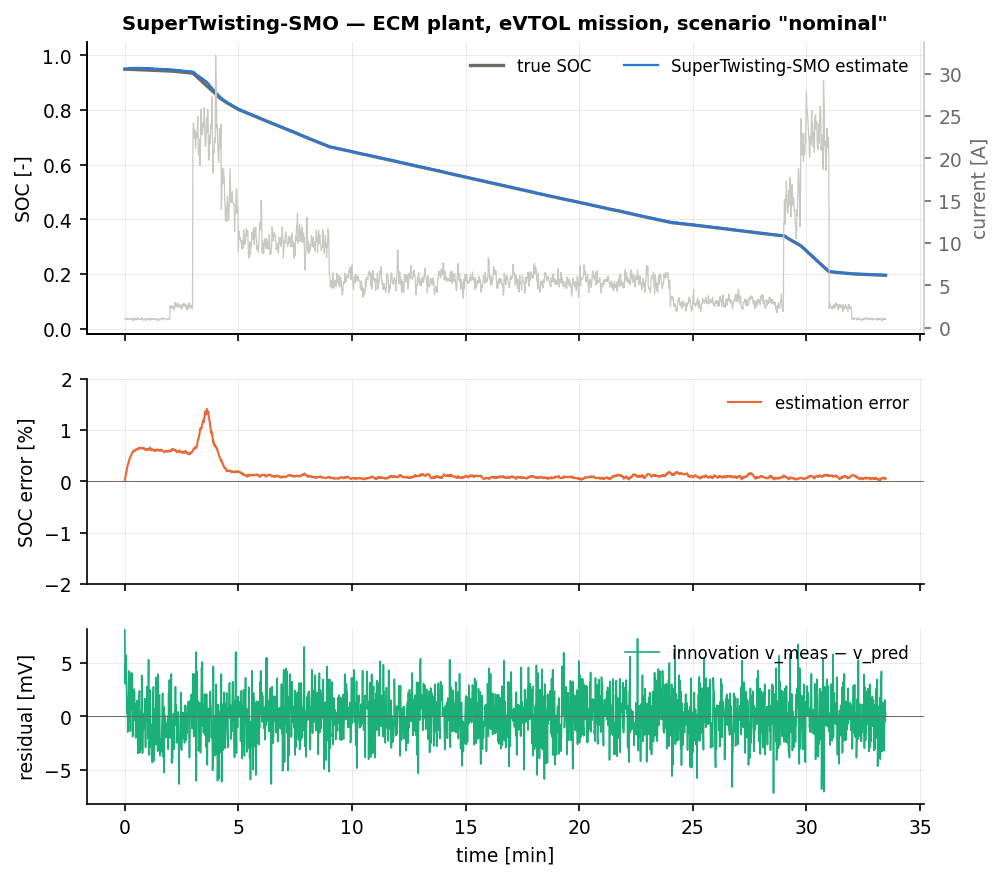
\includegraphics[width=\textwidth]{figures/cell_SuperTwistingSMO_nominal.png}
\caption{SuperTwisting-SMO on the nominal eVTOL mission: true and estimated SOC (top), estimation error with the $\pm 2\sigma$ band when available (middle), voltage residual (bottom).}
\end{figure}
\begin{figure}[H]\centering
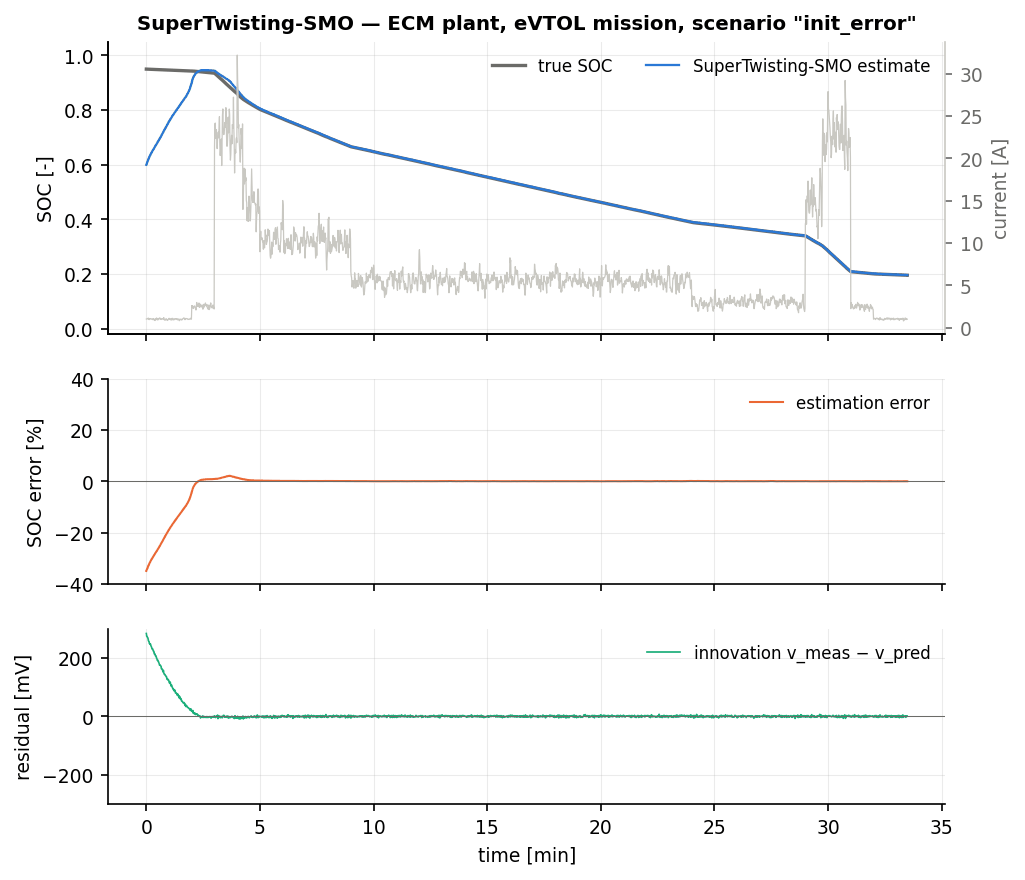
\includegraphics[width=\textwidth]{figures/cell_SuperTwistingSMO_init_error.png}
\caption{SuperTwisting-SMO with a 35\,\% initial SOC error.}
\end{figure}

All numbers are over three seeds.  The observer reaches $\mathrm{rmse}_{ss}=0.0009$ on
\texttt{nominal} --- within a factor of two of the EKF --- for a fifth of the run-time cost and
with a single tuning pair.  It is by a wide margin the cheapest estimator in the family at
$0.14\,\mu$s/step, because it is the only one that never solves a Riccati equation or a placement
problem: there is no gain to design, hence nothing to certify, and the whole scheduling apparatus
of \Cref{sec:lue-schedule} is simply absent.  That is worth noting as a structural advantage and
not only a cost advantage --- this observer was the only one of the twelve that was never
implicated in a seed-dependent failure.

On \texttt{init\_error} it converges in $125$\,s, against $323$--$334$\,s for every
pole-placed or LQE observer in the family; the square-root term is what does it, since it gives a
correction proportional to $|r|^{1/2}$ rather than $|r|$, which is relatively larger when the
residual is small and so shortens the tail of the transient rather than its beginning.  The
clearest demonstration of the integral part is \texttt{combined}: $91$\,s to convergence --- four
to fifteen times faster than anything else here except the PI observer --- with
$\mathrm{rmse}_{ss}=0.0246$, against the EKF's never converging and $0.1244$.

Across the fault scenarios it behaves like a well-tuned linear observer with a slow integrator:
\texttt{outliers} $0.0009$ (the best in the family), \texttt{sensor\_dropout} $0.0009$,
\texttt{noise\_step} $0.0016$ (also the best, and the only observer here that \emph{improves} when
$\sigma_v$ jumps, because the $|r|^{1/2}$ law compresses large residuals), \texttt{cold} $0.0037$.
It is weaker on \texttt{aged\_cell} ($0.0249$) and \texttt{param\_mismatch} ($0.0173$) for the
reason given in \Cref{ch:smo}: the perturbation there is proportional to a current that swings by
a factor of twenty, so it violates the ``slowly varying'' spirit of \eqref{eq:sto-growth}, and no
amount of sliding-mode machinery recovers a parameter that is simply wrong.  A useful detail is
the maximum-error column: $0.014$ on \texttt{nominal} against the Luenberger's $0.006$ --- the
square-root injection is slightly more excitable at small residuals, which is the cost of its
faster tail.

On the single-particle plant it sits at $0.0096$ (\texttt{nominal}) and $0.0512$ (\texttt{cold}),
i.e. about $1.6\times$ the certified LQE observer.  Injecting along a single direction is what
costs it here: the ECM-vs-SPM discrepancy is spread across the RC states, and a one-direction
injection cannot correct them.

\section{Summary}
The super-twisting observer is the best value-for-cycles estimator in this family: two gains, one
direction vector, one square root, $0.14\,\mu$s/step, and accuracy within a factor of two
of an EKF on every well-posed scenario, with a continuous injection and built-in integral action.
Size $k_1,k_2$ from \eqref{eq:sto-cond} or Levant's rule using an estimate of the perturbation
growth $\delta$, normalise the injection direction so that $\mC\bm{\Lambda}=1$, regularise the
$\sgn$ inside the integrator and clamp it.  Do not expect it to fix a wrong capacity or a wrong
$R_0$ --- and if the RC states themselves need correcting (a badly identified impedance), use a
full-state observer instead, because this one only injects along one direction.
